%======================================================================
\NEWSEC
%======================================================================

\subsection{\ssTesting}

\begin{frame}[fragile,label=ss-testing] 
\secframetitle{\ssTesting}
\begin{itemize}
\item \greentext{\url{http://cello-project.org} / \framebox{Regression tests}}
\item \bluetext{Regression tests available in} \redcode{cello-src}
\item \redcode{\$ make test} \bluetext{(takes about 30-60 minutes)}
\item \bluetext{Tests parameter files in} \redcode{cello-src/input}
\item \bluetext{Tests are run in} \redcode{cello-src/test}
\item \bluetext{Test results viewed using}  \redcode{cello-src/test/index.php}
\end{itemize}
\end{frame}

\begin{frame}[fragile] 
\secframetitle{\ssTesting}
\framesubtitle{Enzo-P/Cello Test Results: header table}
\begin{minipage}{2.0in}
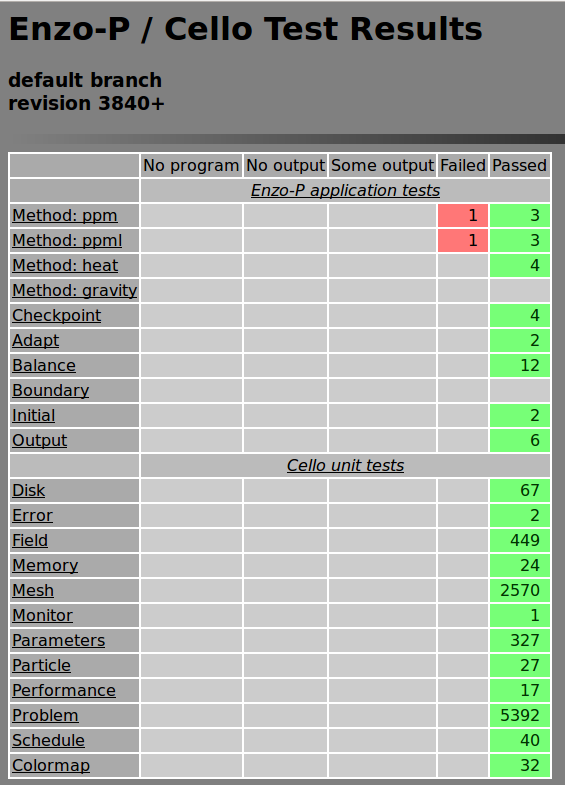
\includegraphics[width=2.0in]{Images/cello-test.png}
\end{minipage} \ 
\begin{minipage}{2.0in}
\begin{itemize}
\item Summary of all tests
\item Columns:
\footnotesize
\begin{enumerate}
\item didn't compile
\item didn't start
\item didn't finish
\item tests failed
\item tests passed
\end{enumerate}
\small
\item Two failed tests expected
\item Sections link to details
\end{itemize}
\end{minipage}
\end{frame}

%----------------------------------------------------------------------

\begin{frame}[fragile] 
\secframetitle{\ssTesting}
\framesubtitle{Enzo-P/Cello Test Results: adaptive mesh refinement}
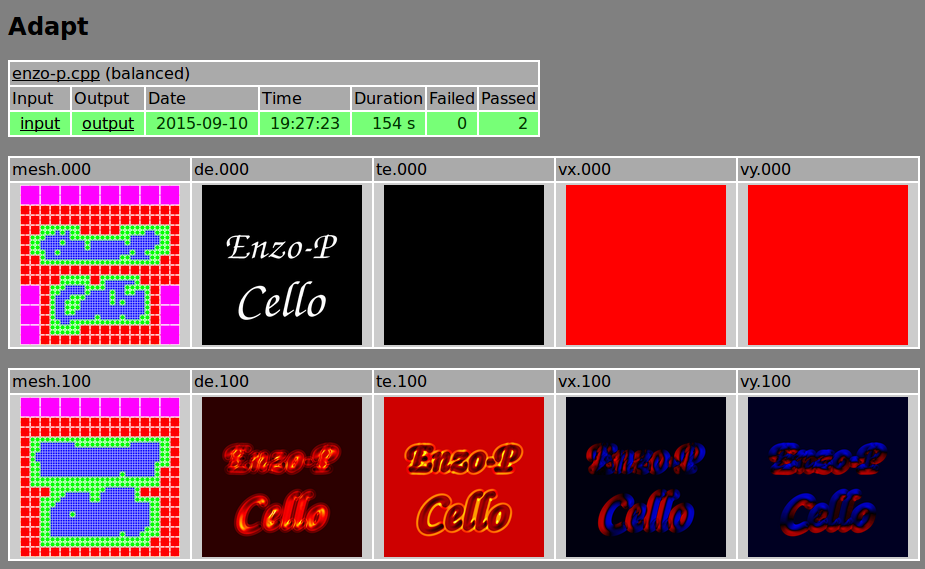
\includegraphics[width=4.0in]{Images/cello-test-2.png}
\end{frame}


\begin{frame}[fragile] 
\secframetitle{\ssTesting}
\framesubtitle{Enzo-P/Cello Test Results: dynamic load balancing}
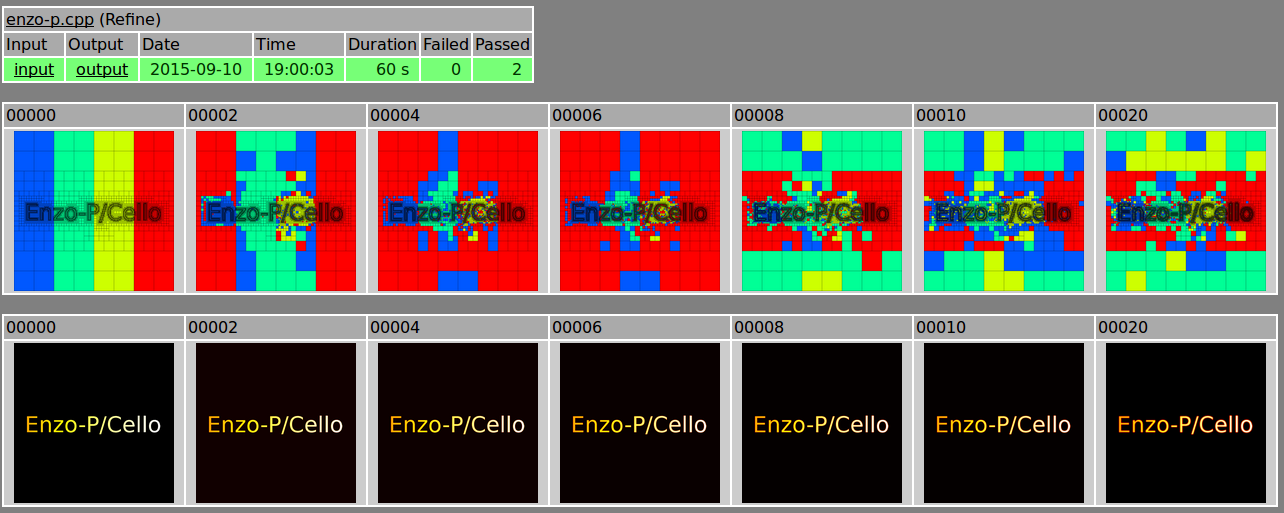
\includegraphics[width=4.0in]{Images/cello-test-3.png}
\end{frame}

